\documentclass[12pt]{article}

% Packages
\usepackage{amsmath, amssymb}
\usepackage{geometry}
\usepackage{graphicx}
\graphicspath{{../../images/}}

\usepackage[colorlinks = true,
            linkcolor = blue,
            urlcolor  = blue,
            citecolor = blue,
            anchorcolor = blue]{hyperref}
\usepackage{enumitem}
\usepackage[backend=biber, style=numeric]{biblatex}
\addbibresource{sba_classification.bib}
\usepackage[skins]{tcolorbox}
\usepackage[T1]{fontenc}
\usepackage[ttdefault=true]{AnonymousPro}
\renewcommand*\familydefault{\ttdefault} %% Only if the base font of the document is to be typewriter style
% Page setup

\geometry{margin=1in}





\begin{document}

\begin{tcolorbox}[halign=flush center]
         \textbf{Analysis of SBA 7a loans}
   
 \end{tcolorbox}

\section{Introduction}
This document provides a descriptive analysis of the SBA 7a loans dataset. Hopefulully, this analysis will illustrate to the reader the importance of doing data analysis and visualization. The most informative feature for this dataset is one that is developed using the notion of a graph. The neighbor hood and geometric landmarks of bad loans are used to predict the likelihood of a loan being bad. It turns out that these are the most informative features. The ideas used to develop these features are discussed in the feature engineering section of this document. They are simple to understand and implement. This analysis is meant to be a starting point for further exploration and understanding of the dataset. Further benefits of doing data analysis and visualization with graph based ideas will be discussed in future work.

\section{Dataset Overview}
\subsection{Data Description}
7a loans are the most common type of SBA loan, designed to help small businesses with financing needs. The dataset includes information on loan amounts, purposes, borrower demographics, and geographic locations. For more details, refer to the official documentation: \href{https://www.sba.gov/partners/lenders/7a-loan-program/types-7a-loans}{SBA 7(a) Loan Data}.
\subsection{Data Source}
The data is sourced from the U.S. Small Business Administration (SBA) and is publicly available for analysis. Please see \href{https://data.sba.gov/dataset/7-a-504-foia}{SBA 7(a) Loan Data} for access.
\subsection{Data Fields}
Please refer to the dataset documentation for a comprehensive list of fields. Key fields include:
\begin{itemize}
    \item Loan Amount
    \item Loan Purpose
    \item Borrower Demographics
    \item Geographic Location
    \item Approval Status
    \item Date of Loan
    \item Lender Information
    \item Business Type
    \item Industry Classification
    \item Current Status of Loan    
\end{itemize}

\section{Data Cleaning}
The following steps were taken to clean the dataset:
\begin{itemize}
    \item Inconsistent data: There were a small set of loans where the disbursement date was after the paid in full date. These loans were removed from the dataset.
    \item Data Type Assignment: Ensured all fields have appropriate data types (e.g., dates, numeric values).
    \item Support Check for Categorical Variables: Verified that categorical variables had minimum support to ensure that we can draw meaningful conclusions - i.e., generalization is possible. The geographical attributes with low support were hierarchical in some cases. For example, zip code and NAICS code. In these cases, the higher level of the hierarchy was used. This can be done by applying a mask to the zip code or NAICS code. For example, using only the first 3 digits of a zip code or the first 2 digits of a NAICS code. 
    \item Derived Attribute Creation: An attribute that captures the number of payments on the loan was created.
\end{itemize}
Please see the \href{https://github.com/rajivsam/descriptive_analytics/blob/main/notebooks/sba_loans.ipynb}{data cleaning notebook} for implementation details.

\section{Data Partitioning}
The dataset was partitioned into training, validation, and test sets. The training set was used for analysis, feature engineering, and model training. The validation set was used for hyperparameter tuning and model selection. The test set was reserved for final evaluation of the model's performance. 


\section{Feature Engineering}
The categorical variables were encoded using a target encoding scheme. Please see \href{https://github.com/rajivsam/descriptive_analytics/blob/main/notebooks/sba_loan_numeric_enc.ipynb}{this notebook} for the implementation. The target variable is highly imbalanced, with a small percentage of loans being classified as bad. To address this, the following feature were engineered: :
\begin{itemize}
    \item Risky Neighborhood Feature: A $k$ nearest neighbor graph of the loans that were charged off was constructed. The loans in the $k$ nearest neighbor graph were considered a \emph{risk region}. A loan is considered to be in a risky neighborbood if its nearest neighbor is in the risk region. This feature was found to be highly informative. Note that the \emph{risk region} is constructed using only the training data.
    \item Distance to Charged Off Loan Clusters: The charged off loans were clustered using a density based clustering algorithm \cite{ester1996density}. The $\epsilon$ parameter and the minimum number of samples parameters were chosen so that the number of clusters was two. The centroids of the clusters were computed. The distance from each loan to the centroids of the clusters was computed. This feature was also found to be highly informative. The number of clusters can be tuned as a hyperparameter. Note that the clusters are constructed using only the training data. Tuning the number of clusters is a hyperparameter that can be done using the validation set and is not done in this analysis. It is left for future work and definitely worth exploring.
\end{itemize}
Please see \href{https://github.com/rajivsam/descriptive_analytics/blob/main/notebooks/sba_bad_borr_graph_ctor.ipynb}{this notebook} for the implementation of the feature engineering.

\section{Modeling Approach}
Since the dataset is highly imbalanced, we cannot use the conventional accuracy metric to evaluate the model. The threshold for classifying an instance as positive or negative can be tuned to achieve a desired balance between precision and recall. In a balanced dataset, the threshold is typically set to 0.5. The imbalance provides very little room for errors in probablity of a chargeoff. To mitigate this, a probablity calibration model is used \cite{platt1999probabilistic}. The calibration model calibrates the probablity of a chargeoff that is output by the classifier.

The precision of a classifier is the fraction of true positives among all instances classified as positive. The recall of a classifier is the fraction of true positives among all actual positive instances. In applications such as marketing, precision is often more important than recall. This is because false positives are what we need to tune to control costs and profits. In contrast, in applications such as fraud detection or health cate, recall is often more important than precision. This is because false negatives are what we need to tune to control costs and profits.

This application falls under the latter category. We want to catch as many bad loans as possible. This is because the cost of a false negative (i.e., a bad loan that is not identified) is much higher than the cost of a false positive (i.e., a good loan that is identified as bad). 

A random forest classifier \cite{breiman2001random} was used for this analysis. The classifier developed using the training set was evaluated on the validation set. For this analysis, a recall of $0.9$ was chosen as the acceptable level of recall. We hope to catch $90\%$ of the bad loans. The threshold for this level of recall was used to evaluate the model on the test set.

The precision recall-curve for the validation set is shown in the figure \ref{fig:pr_curve}.
\begin{figure}
    \centering
    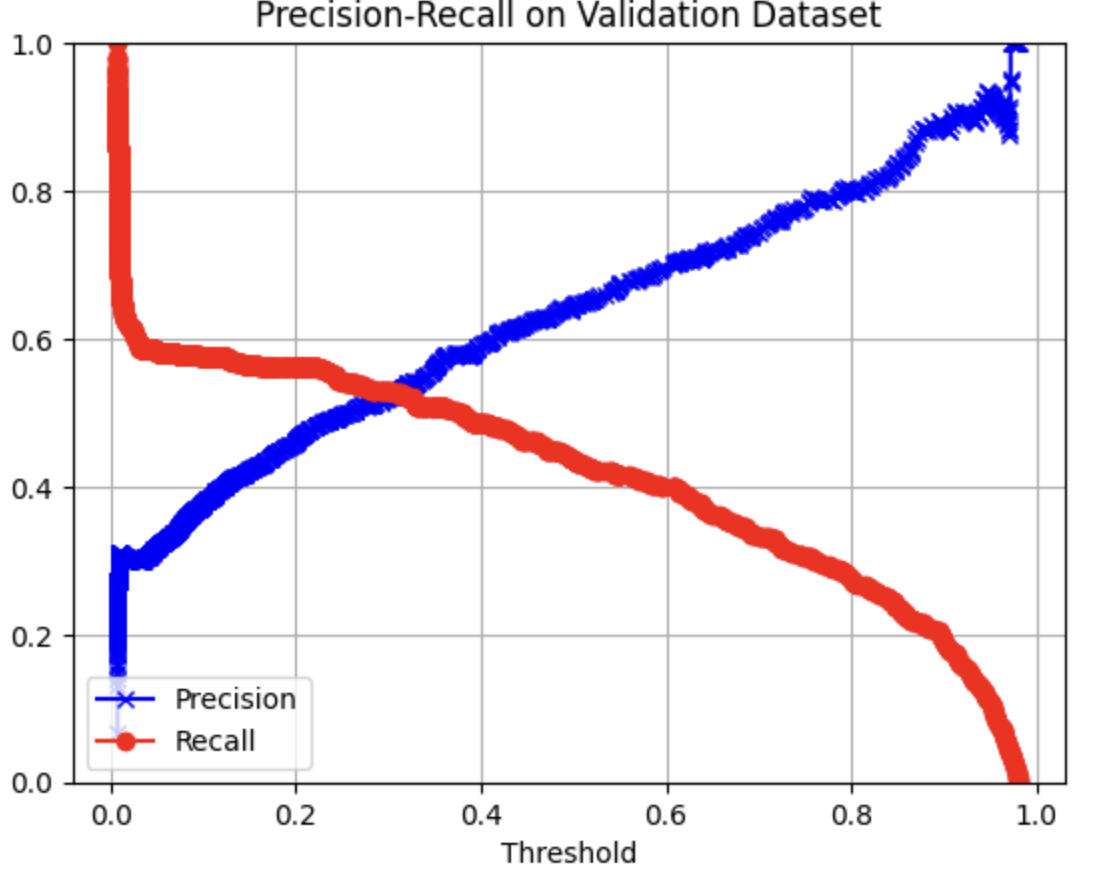
\includegraphics[width=0.7\textwidth]{sba-precision-recall-curve-val.png}
    \caption{Precision Recall Curve for the validation set}
    \label{fig:pr_curve}
\end{figure}

\section{Results}
The results of model evaluation on the test set are shown in figure \ref{fig:test_perf}. The results show that we are able to capture $85\ \%$ of the bad loans with the threshold determined using the validation set. The precision is $0.17$. This means that $17\%$ of the loans that are classified as bad are actually bad. This is not a bad    result given the imbalance in the dataset. The model can be further improved by tuning the hyperparameters. It is important to note that the number of loans that are tagged as bad by the model is relatively small. Only about $31\ \%$ of the loans are tagged as bad. This is a manageable number for further investigation. Nearly $70\%$ of the loans do not need further investigation. This is a significant reduction in the number of loans that need to be investigated. This is the main benefit of using a model like this. It helps reduce the workload of the analysts. The model can be further improved by tuning the hyperparameters and exploring other features. This is left for future work.

\begin{figure}
    \centering
    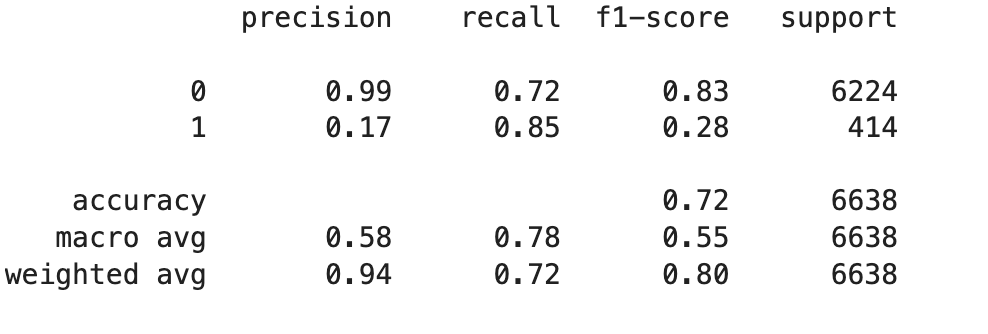
\includegraphics[width=0.7\textwidth]{sba-test-set-perf.png}
    \caption{Performance on the test set}
    \label{fig:test_perf}
\end{figure}

The classifier and scoring analysis is available 
\href{https://github.com/rajivsam/descriptive_analytics/blob/main/notebooks/sba_bad_loans_classifier.ipynb}{in this notebook}. Since probablities of charage offs can be obtained from the model, it is possible to factor costs and benefits into the decision making process. This is not explored in this example, but the framework is flexible enough to accomodate this, see \cite{verbraken2012novel} for more details on cost sensitive learning. 

\section{Observations and Insights}


\begin{figure}[!ht]
    \centering
    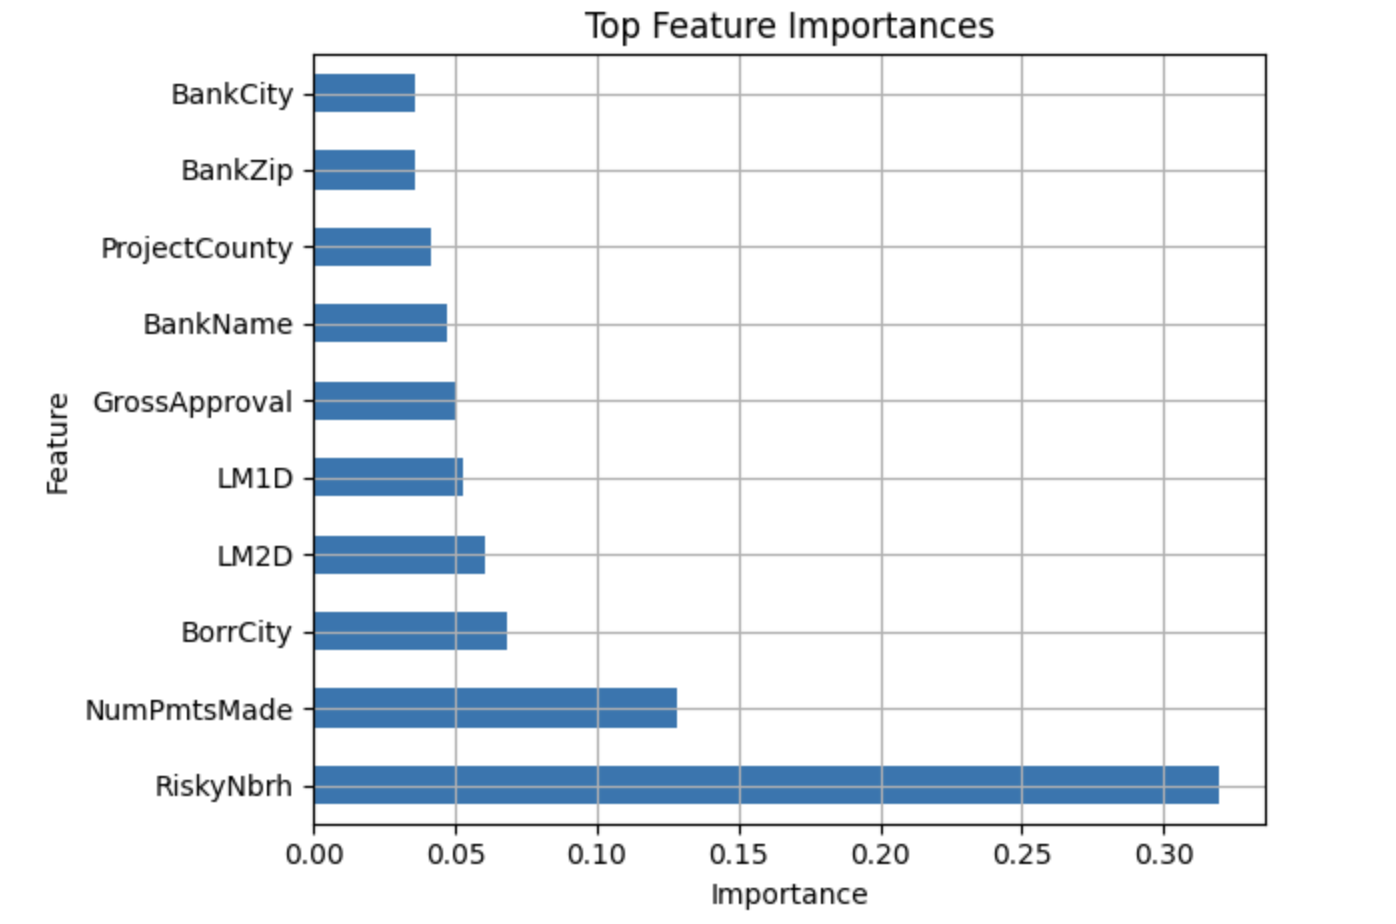
\includegraphics[width=0.7\textwidth]{sba-feature-importances.png}
    \caption{Feature Importance Plot}
    \label{fig:feat_imp}
\end{figure}
The feature importance plot is shown in figure \ref{fig:feat_imp}. This example underscores the importance of data analysis in the development of machine learning models. The most informative features were developed using the notion of a graph. The neighborhood and geometric landmarks of bad loans were used to predict the likelihood of a loan being bad. These features are simple to understand and implement. This analysis is meant to be a starting point for further exploration and understanding of the dataset. Further analysis of the charged off loans may reveal other features that we could exploit. This is a real world dataset and modeling is an iterative process. Hopefully, this convinces the reader of the importance of the data analysis step in the machine learning pipeline. Not only is the model better, using features that are meaningful and interpretable make it possible to explain the model to stakeholders. It helps build trust. This is crucial in real world applications.

\printbibliography

\end{document}